
% This LaTeX was auto-generated from MATLAB code.
% To make changes, update the MATLAB code and republish this document.

\documentclass{article}
\usepackage{graphicx}
\usepackage{color}

\sloppy
\definecolor{lightgray}{gray}{0.5}
\setlength{\parindent}{0pt}

\begin{document}

    
    
\subsection*{Contents}

\begin{itemize}
\setlength{\itemsep}{-1ex}
   \item 6.6A
   \item 6.6B
   \item a)
   \item b)
   \item c)
   \item d)
   \item e)
   \item 6.6C
   \item a)
   \item c
\end{itemize}


\subsection*{6.6A}

\begin{verbatim}
load('exercise_fMRI_small.mat');
\end{verbatim}


\subsection*{6.6B}



\subsection*{a)}

\begin{verbatim}
s1 = zeros(1,50);
s1(25) = 1;
\end{verbatim}


\subsection*{b)}

\begin{verbatim}
c1 = conv(s1, hrf);
\end{verbatim}


\subsection*{c)}

\begin{verbatim}
c1t =  0:3.22: 3.22*(length(c1)-1);
s1t = 0:3.22: 3.22*(length(s1)-1);

plot(c1t, c1, 'DisplayName', 'Convolution Signal', 'LineWidth', 1);
hold on;
plot(s1t, s1, 'DisplayName', 'Stimulus Presentation', 'LineWidth', 1 );
legend
xlabel('time (s)');
xlim([50 125]);
ylabel('amplitude');
\end{verbatim}

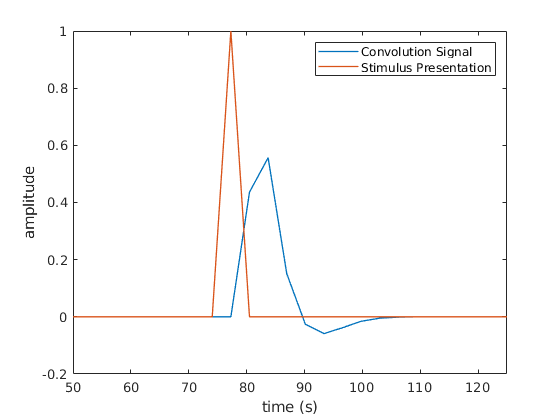
\includegraphics [width=4in]{ex6_6_01.eps}


\subsection*{d)}

\begin{par}
the new hrf doesn't reach as high as the one in 6.2B, probably the result of convolution with a different HRF vector
\end{par} \vspace{1em}


\subsection*{e)}

\begin{par}
the signal spike happens about 6.5 seconds after the stimulus, and it is returned to baseline level at 109.48 seconds, about 29 seconds after its onset
\end{par} \vspace{1em}


\subsection*{6.6C}



\subsection*{a)}

\begin{verbatim}
hold off;

nrscans = length(bold);
D = [];
conditions = ["fix", "stat", "att", "natt"];
for condition = conditions
    con_idx = eval(condition);
    condition_stimuli = zeros(nrscans, 1); % make a zeros vector
    condition_stimuli(con_idx) = 1; % populate zeros vector with index of stimulus presentation
    D = [D condition_stimuli];
end

time = 0:3.22: 3.22*(length(bold) -1);

subplot(4,2,2:2:8);
imagesc(D);
colormap gray;
title('Design Matrix');
ylabel('time (s)');
xlabel('Regression');

idx = 1;
for i=1:2:7
    subplot(4,2,i);
    plot(time, D(:,idx));
    ylim([-0.1 1.1]);
    xlim([0 time(end)]);
    title(strcat("condition ", conditions(idx)));
    idx = idx + 1;
end
xlabel('time (s)');
\end{verbatim}

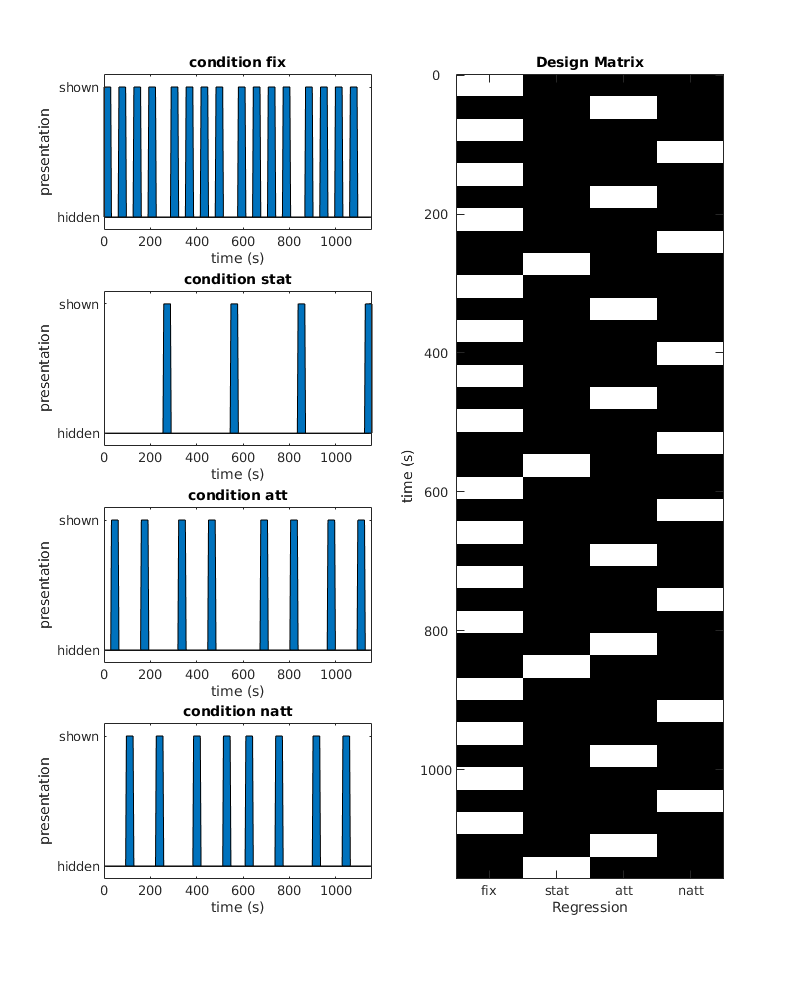
\includegraphics [width=4in]{ex6_6_02.eps}


\subsection*{c}

\begin{par}
condition \ensuremath{|}  number of presentations fix       \ensuremath{|} 16 stat      \ensuremath{|} 4 att       \ensuremath{|} 8 natt      \ensuremath{|} 8
\end{par} \vspace{1em}



\end{document}

